\chapter{PAGES WITH A FIGURE, A TABLE AND A EQUATION}
\section{Figure Placement and Size}

Figures need to be within the set text margins and be large enough to read (1.5mm or about 7 pt type). You need spacing above and below the figure or table that is more than the spacing of the text. At least a triple (or three single) spaces is needed. Figures do not need to have the same size or style of type in them.

\section{Figure Titles}
The style of the figure titles needs to be \textbf{consistent} for all the figures. This includes bold or not, italics, abbreviations, (Fig.1 vs Figure 1, for instance), vertical spacing, flush or centered on the page. This does not include type size and style, which can vary from figure to figure. See Figure \ref{fig:exampleA} and %\ref{fig:exampleB} and
% \ref{fig:exampleC} 
caption for information on figure numbering and spacing.

\begin{figure}[!htb]
\centering
\begin{minipage}{0.45\textwidth}
		\begin{center}
		
\includegraphics[width=\textwidth]{graphic/TAMUthesis_exampleA.png}
%		\caption[short title for exampleA]{The figures can be numbered consecutively throughout the thesis (1, 2, 3, 4, etc) or \textbf{numbered by chapter (1-1, 1-2, 2-1, etc.)}. (A) Each figure should be referred to by that number within the text, within 1 $\frac{1}{2}$ pages of the figure.}
%		\label{fig:exampleA}
		\end{center}	
\end{minipage} %
\begin{minipage}{0.45\textwidth}
			\begin{center}
			
\includegraphics[width=\textwidth]{graphic/TAMUthesis_exampleB.png}
		%	\caption[short title for exampleB]{(B) The figures can be put on a separate page from the text, but if they are incorporated into the text, they must be offset by at least a triple space above and below. The following text are typed in to fill in the blank spaces of the mini page.}
			%to place a caption outside a floating environment, use \captionof from caption package
%			\label{fig:exampleB}
			\end{center}	
	\end{minipage}
	\caption[\protect\vspace{-2.8ex}{The Entire Title Up To The First Period Must Be Included In The List.}]{The entire title up to the first period must be included in the List. Lists of Figures and Tables must agree word for word with figure and table titles in the text. The figures can be numbered consecutively throughout the thesis (1, 2, 3, 4, etc) or \textbf{numbered by chapter (1-1, 1-2, 2-1, etc.)}. (A) Each figure should be referred to by that number within the text, within 1 $\frac{1}{2}$ pages of the figure.(B) The figures can be put on a separate page from the text, but if they are incorporated into the text, they must be offset by at least a triple space above and below.(C) Figures must fit within the normal page margins. Figure captions are not considered regular text, and so may be a different font size and may be single spaced. Each figure must have a unique caption, and captions, up to the first period, must be included in the List of Figures. Though larger size font for picture are allowed, it needs to be consistency throughout the whole thesis.}
	\label{fig:exampleA}
\end{figure}
		

\begin{Contfigure}[!htb]
\captionsetup{list=off}	%disable lof display this figure name as continued
\begin{center}
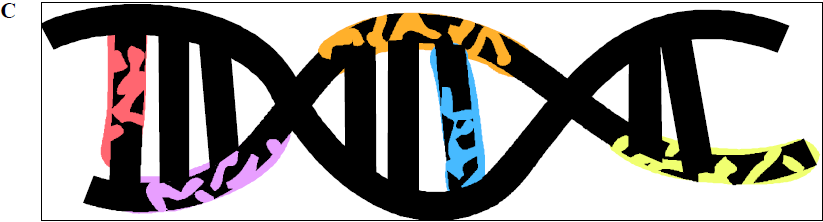
\includegraphics[width=\textwidth]{graphic/TAMUthesis_exampleC.png}
\caption{}
\label{fig:exampleC}
\end{center}
\end{Contfigure}
%line must be added after continued figure
\renewcommand{\thefigure}{\arabic{chapter}.\arabic{figure} }
%end of line

\section{Continued Figures}
It's not recommended to use continued figures in this \LaTeX ~document since figure/table numbering increases automatically. But if you would like to use it, refer to Figure \ref{fig:UltrasoundSystem1} for how Continued Figure works.
 
\begin{figure}[!hbp]
\begin{center}
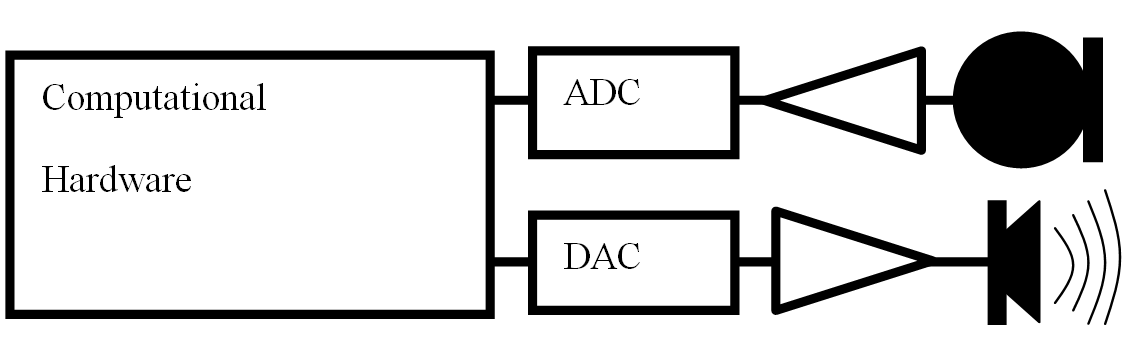
\includegraphics[width=\textwidth]{graphic/UltraSoundSystem_Simple.PNG}
\caption[\protect\vspace{-2.8ex}{Please Check  This Figure's Implementation Code To See How To Meet University Requirement Of Single Space Long Figure/Table Titles.}]{Please Check  This Figure's Implementation Code To See How To Meet University Requirement Of Single Space Long Figure/Table Titles.}
\label{fig:UltrasoundSystem1}
\end{center}
\end{figure}
\begin{Contfigure}[!hbp]
\captionsetup{list=off}	%disable lof display this figure name as continued
\begin{center}
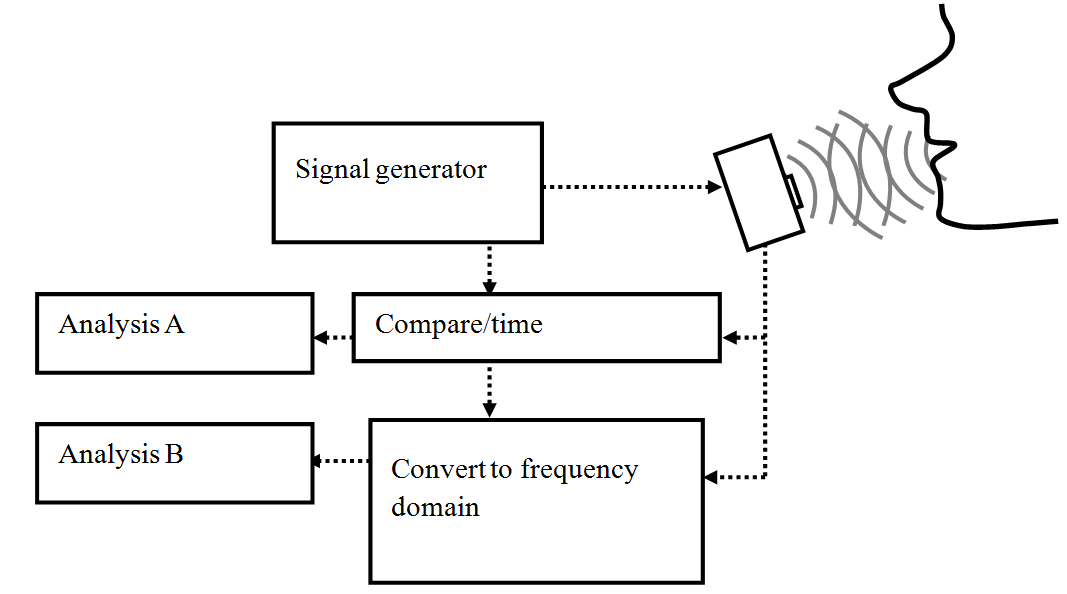
\includegraphics[width=\textwidth]{graphic/UltraSoundSystem_Flow.PNG}
\caption{}
%A diagram showing how the reflected signal is processed inside the system
\label{fig:UltrasoundSystem2}
\end{center}
\end{Contfigure}

Figure \ref{fig:UltrasoundSystem2} provides high level blocks of the system.

\begin{figure}[!hbp]
\begin{center}

\includegraphics[width=0.5\textwidth]{graphic/primaryWhiteMaroon_RGB.jpg}
\caption[\protect\vspace{-2.8ex}{Figure Name Should Have Consistent Behavior Along This Document.}]{Figure Name Should Have Consistent Behavior Along This Document.}
\label{fig:testExample2}
\end{center}
\end{figure}

\section{Table Placement, Size and Table Title}
As with figures, tables placed in text need to be separated from the test by at least a triple space. Table titles can be numbered by chapter or numbered consecutively throughout the thesis. Their titles need to be consistent, as figure titles. If you have a continued table, repeat the column headings. Please see Table \ref{tab:exampleA} %and \ref{tab:exampleB}
as a reference. Free software is available on-line to convert excel table into \LaTeX ~table format, please refer to 

\verb|http://www.ctan.org/pkg/excel2latex|.

\begin{table}[h]
	\begin{center}
	\caption{Results From Experimental And Control Runs}
	\label{tab:exampleA}
	\begin{tabular}{||c|c|c|c|c||}		
		\hline
		Species  	&  	Experiment 1	&  Experiment 2  	&  	Control 1 	& 	Control 2	\\	\hline
		Cow	   	&  	\verb|+|	&  \verb|-|		&	\verb|-|	&	\verb|+|	\\	\hline
		Brown Horse	&	\verb|-|	&	\verb|+|	&	\verb|-|	&	\verb|-|	\\	\hline
		Gray Cow	&			&			&			&			\\	\hline
		White House	&	\verb|-|	&	\verb|+|	&	\verb|+|	&	\verb|-|	\\	\hline
		Tan Cow	&	\verb|+|	&	\verb|-|	&	\verb|-|	&	\verb|+|		\\	\hline
	\end{tabular}
	\end{center}
\end{table}


%the line below must be added if using continued table
\renewcommand{\thetable}{\arabic{chapter}.\arabic{table} Continued.}
\addtocounter{table}{-1}
%end of line	
% or use \begin{Conttable}	
\begin{table}[h]
	\captionsetup{list=off}	%disable lof display this figure name as continued
	\begin{center}
%	\caption{Results From Experimental And Control Runs}
	\caption{}
	\label{tab:exampleB}
	\begin{tabular}{||c|c|c|c|c||}		
		\hline
		Species  	&  	Experiment 1	&  Experiment 2  	&  	Control 1 	& 	Control 2	\\	\hline
		White Cow   	&  	$+$		&  	$-$		&	$-$		&	$+$		\\	\hline
		Spotted Pig	&	$+$		&	$+$		&	$+$		&	$-$		\\	\hline
		White Pig	&	$+$		&	$-$		&	$-$		&	$-$		\\	\hline
		Brown Pig	&			&	$+$		&	$+$		&	$-$		\\	\hline
		Gray Pig	&	$+$		&	$-$		&	$-$		&	$+$		\\	\hline
		Black Pig	&	$+$		&	$-$		&	$-$		&	$+$		\\	\hline
	\end{tabular}
	\end{center}
\end{table}
\renewcommand{\thetable}{\arabic{chapter}.\arabic{table}}

For more table format, please refer to Table \ref{tab:Cosine2Phase} for more information.
\section{Equations}
%Equ. \ref{equ:x_rotate1}, \ref{equ:y_rotate1} and \ref{equ:Euler} are referred here.
The following format is recommended to be used to display. The equation can be referred as Equ. \eqref{equ:secondRepeat}. Please pay special attention when using \textbf{equation} environment for it will cause extra large vertical space in the \LaTeX ~ documents. Use other environment like \textbf{align} to write multi-line equations. When equation environment is applied, please don't leave a blank line before it. 

When refer to any equations, command \verb|\eqref{}| [Equ. \eqref{equ:secondRepeat}] instead of \verb|\ref{}| [Equ. \ref{equ:secondRepeat}] is preferred. 
%\begin{center}
%\begin{equation}
%x^{'} = x \cdot cos(a) - y \cdot sin(a)  \label{equ:x_rotate1}
%\end{equation}
%%reduce vertical space between equations
%\begin{equation}
%y^{'} = y \cdot cos(a) + x \cdot sin(a)  \label{equ:y_rotate1}
%\end{equation}
%\begin{equation}
%e^{ja}=cos(a)+j \times sin(a)	\tag{Euler's Identity} 	\label{equ:Euler}
%\end{equation}
%\end{center}
\begin{align}
x^{'} 	& 	= x \cdot cos(a) - y \cdot sin(a)  	   			\\
y^{'}  &	= y \cdot cos(a) + x \cdot sin(a)  				\\
e^{ja} & 	=cos(a)+j \times sin(a)	 	
\label{equ:secondRepeat}
\end{align}

The test here is to show the vertical spacing after the equations. 
%%%%%%%%%%%%%%%%%%%%%%%%%%%%%%%%%%
%\setlength{\belowdisplayskip}{1em} \setlength{\belowdisplayshortskip}{1em}

\pagebreak[4] %intentionally to display the two equations below on the same page for illustration purpose.
\section{Equation Vertical Spacing}
Please read the two Equ. \eqref{equ:WADequ} and \eqref{equ:WADequ2} below to have a brief idea about equation vertical spacing. The usage of equation environment \textbf{array} is tested as well. In the code implemented, no extra line is provide between the text and equation in Equ. \eqref{equ:WADequ}. This provides tight vertical spacing as shown, however, adding the extra line command will cause un-balanced vertical spacing before/after the equation. The reason seems fundamental and unchangeable under~\LaTeX. A temporary local fix is provided in the code below for Equ. \eqref{equ:WADequ2}
%\\	%you can try to uncomment the \\ at the beginning of the line to see the effect.
\begin{equation}
WAD(S_{n}) = \Bigg\{ 
\begin{array}{ccc}
+1 & if &  E(S_{n}) >  \varepsilon_{2}      	\\
-1 & if &  E(S_{n}) < \varepsilon_{1}       \\
sign(zcr(S_n)) - \varepsilon_{zcr} & if &  \varepsilon_{1} \le E(S_{n}) \ge \varepsilon_{2}       \\
\end{array}
\label{equ:WADequ}
\end{equation}
This line is to separate the two equations below and above. The equation below has a temporary local solution to adjust the vertical spacing before the equation. Please notice the difference of the code implemented. The easiest way is to do as Equ. \eqref{equ:WADequ} do.
\\[-2ex]	%you can try to uncomment the \\ at the beginning of the line to see the effect.
\begin{align}
WAD(S_{n}) = \Bigg\{ 	& % the & in front is for align environment
\begin{array}{ccc}
+1 & if &  E(S_{n}) >  \varepsilon_{2}      	\\
-1 & if &  E(S_{n}) < \varepsilon_{1}       \\
sign(zcr(S_n)) - \varepsilon_{zcr} & if &  \varepsilon_{1} \le E(S_{n}) \ge \varepsilon_{2}       \\
\end{array}
\label{equ:WADequ2}
\end{align}
\\
Test text for vertical spacing test only.

\section{Other Information In This Document}
All requirements in this document comes from OGAPS Thesis manual, which you can download from \href{http://ogapstest.tamu.edu/New-Current-Students/Thesis-and-Dissertation-Services/Prepare-Your-Document/#0-ResourcesforPreparation}{OGAPS Current Students Thesis/Dissertation Service web page}. After this section, most content in this document repeats what the manual thesis say.  You might notice there are plenty of non-meaningful text appearing in this document. They are for the purpose of testing the structure of toc/lof/lot, Appendix and Word `Page` etc. You can just ignore them and use the blank template provided. However, code examples in this document might be useful if you are not sure about the implementation of certain features in your thesis and you can refer to this document then.
\section{Another Test Section}
The section title is to test the toc only, no other purpose.

 \begin{figure}[!hbp]
\begin{center}

\includegraphics[width=0.4\textwidth]{graphic/logoTAMU.jpg}
\caption[\protect\vspace{-2.8ex}{You Can Choose Your Style for Figure Title, But Please Keep Consistent Throughout The Document.}]{You Can Choose Your Style for Figure Title, But Please Keep Consistent Throughout The Document.}
\label{fig:testExample4}
\end{center}
\end{figure}

\section{Another Test Section 3}
The section title is to test the toc only, no other purpose.

\section{Another Test Section 4}

The section title is to test the toc only, no other purpose.
 \begin{figure}[!htbp]
\begin{center}

\includegraphics[width=0.4\textwidth]{graphic/TAM_Logo1.png}
\caption{TAMU Logo}
\label{fig:testExample1}
[Picture for test lof only, no other purpose]
\end{center}
\end{figure}
 
\section{Another Test Section 5 \& 6}

Just a test section. 
\begin{figure}[!hbp]
\begin{center}

\includegraphics[width=0.3\textwidth]{graphic/LoneStarLogo_WhiteTexas.png}
\caption{In This Document, Figure Title Keeps First Character Capital.}
\label{fig:testExample3}
\end{center}
\end{figure}

